\chapter{卒論っぽいサンプルその1 from K.K 2020}

誰かの卒論の考察部分のみを移行してみた例

\section{はじめに}
ここでは第4章のシミュレーション結果について旋回性能を表す代表値で評価した結果をふまえて,実際の航走試験の航路と推定航路の誤差の原因に関して考察をする.またその誤差の軽減方法に関しても提案し検討する. 

\section{シミュレーション結果の考察}
ケーススタディでおこなった35°旋回試験(右旋回)のシミュレーション結果に焦点を当てて考察する.ケーススタディでは操縦流体力微係数の推定区間として安定して旋回している区間(180.00 [sec] - 245.50[sec])を用いた.しかしその区間で推定した操縦流体力微係数を使用したシミュレーション結果に,船が動き始めてから180.00[sec]程度までの区間において誤差が生じていることが4.5.2.1より判明した.

\subsection{推定区間による誤差}
以上の結果から誤差が生じている区間においてケーススタディで推定した操縦流体力微係数では推定航路に誤差が生じると考えられる.そこで提案手法で述べた安定して旋回している区間を用いて操縦流体力微係数を推定するのではなく,推定区間を船体運動の変化に合わせて分割し,それぞれの区間において操縦流体力微係数を推定する.その推定値をそれぞれの区間で適用し,シミュレーションすることで推定航路の誤差を軽減できるかを検討し考察する.具体的な分割区間は操縦運動パラメータが安定して直進のような運動をしている時間(143.25[sec])から舵角を設定角の35°まで変更した時間(162.00[sec])までの区間と,そこから操縦運動パラメータの変化が収まり,安定して旋回をし始めたと判断できる時間 (180.00[sec])までの区間とそれ以降の区間の3区間とする.

\begin{itemize}
	\item 143.25[sec] – 162.00[sec] :直進のような運動で操縦運動パラメータが安定している区間
	\item 	162.00[sec] – 180.00[sec] :舵角35°で旋回し始め針路が安定していない区間
	\item 180.00[sec] - 245.50 [sec] :安定して旋回運動している区間
\end{itemize}

この3区間でそれぞれ操縦流体力微係数を推定し,分割した区間ごとにシミュレーションをおこない,推定航路の誤差を検討する.3区間目の180.00[sec] - 245.50 [sec]は当初の提案した推定区間であり操縦流体力微係数はケーススタディで用いた値と同一である.\tbref{tb:5-1}にそれぞれ分割した区間で推定した値を示す.

\begin{table}[htbp]
 \caption{Split and estimated results}
 \label{tb:5-1}
 \centering
  \begin{tabular}{crrr}
   \hline
   分割区間[sec] & 143.25 – 162.00 & 162.00 – 180.00 & 180.00 – 245.50 \\
   \hline \hline
   $X_0$ & -0.0024 & -0.0136 & -0.0425 \\
   $X_{\beta\beta}$ & 0.0109 & 0.0005 & 0.0103 \\
   $X_{\beta\gamma}$ & 0.0392 & 0.0011 & 0.0312 \\
   $X_{\gamma\gamma}$ & -0.0064 & -0.0078 & -0.1058 \\
   $X_{\beta\beta\beta\beta}$ & 0.0026 & 0.0001 & 0.0027 \\
   $Y_{\beta}$ & 24.78 & 11.29 & 25.66 \\
   $Y_{\gamma}$ & 0.6590 & -1.095 & -6.880 \\
   $Y_{\beta\beta\beta}$ & -1075 & 872.0 & -83.91 \\
   $Y_{\beta\beta\gamma}$ & 1062 & -396.1 & 25.64 \\
   $Y_{\beta\gamma\gamma}$ & -273.4 & 74.05 & 26.33 \\
   $Y_{\gamma\gamma\gamma}$ & 12.68 & -3.642 & -1.357 \\
   $N_{\beta}$ & 0.1479 & 0.4818 & 0.1302 \\
   $N_{\gamma}$ & -0.4670 & -0.2901 & -0.0557 \\
   $N_{\beta\beta\beta}$ & 4.081 & -14.34 & -0.1061 \\
   $N_{\beta\beta\gamma}$ & -8.672 & 5.752 & 0.0217 \\
   $N_{\beta\gamma\gamma}$ & 2.694 & -0.7574 & -0.0299 \\
   $N_{\gamma\gamma\gamma}$ & 0.2528 & -0.0890 & -0.0230 \\
   \hline
  \end{tabular}
\end{table}

これらの操縦流体力微係数を用いて航路シミュレーションした結果を\figref{fig:5-1_png},\figref{fig:5-2_png},\figref{fig:5-3_png}に示す.グラフには推定区間を分割した推定航路(Split-Estimation),実際の35°旋回試験の航路(Ship 1)とケーススタディでおこなった推定航路(case 1)を描写した.また,推定航路の誤差をわかりやすくするためにそれぞれの区間の初期値を実際の35°旋回試験(右旋回)データの値にそろえた.

\begin{figure}[htbp]
    \centering   
    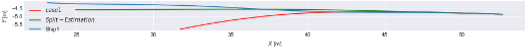
\includegraphics[width=0.5\textwidth]{./img/5-1.png}
    \caption{Sample data and split estimated results (143.25s – 162.00s)}
    \label{fig:5-1_png}
\end{figure}

\begin{figure}[htbp]
    \centering
    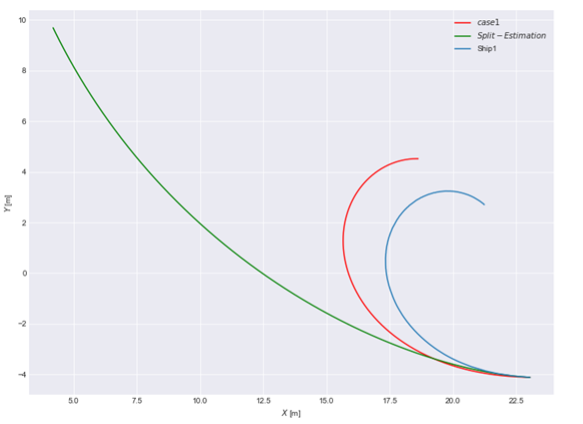
\includegraphics[width=0.5\textwidth]{./img/5-2.png}
    \caption{Sample data and split estimated results (162.00s – 180.00s))}
    \label{fig:5-2_png}
\end{figure}

\begin{figure}[htbp]
    \centering
    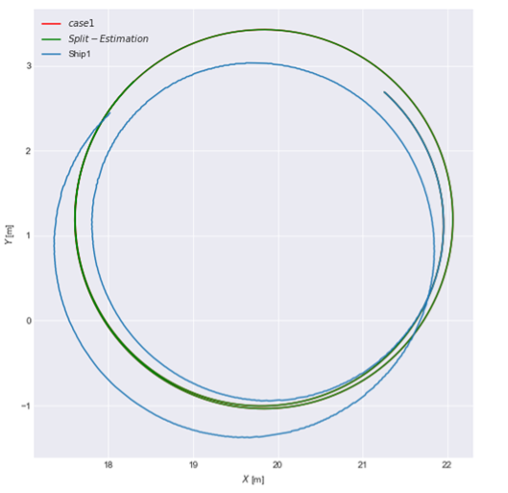
\includegraphics[width=0.8\textwidth]{./img/5-3.png}
    \caption{Sample data and split estimated results (180.00s – 245.50s)}
    \label{fig:5-3_png}
\end{figure}

\subsubsection{推定区間のパラメータによる誤差}
舵角を35°に変更した直後の区間である162.00[sec] – 180.00[sec]でのシミュレーション結果\figref{fig:5-2_png}いて考察する.この区間は推定区間を分割して推定した航路(Split-Estimation)が実際の35°旋回試験の航路(Ship1)と大きく異なっていることがわかる.この区間ではケーススタディでおこなった推定航路(case 1)の方が実際の航路(Ship1)に近い結果となった.原因として考えられることはこの区間(162.00[sec] – 180.00[sec])は操舵をおこなった直後の区間であり針路が安定していなく,操縦運動パラメータが大きく変化している区間であり,本研究では流体力式(3.1)から最小二乗法を用いて操縦流体力微係数を推定しているため,この大きく変化する操縦運動パラメータを取得する際に誤差が生じ,結果としてこの区間の流体力$X_H$,$Y_H$,$N_H$算出時に誤差が生じたものだと考える.以上より推定に使用する区間には操縦運動パラメータが安定して一定な区間が良いということが確認できた.

これはZ試験の航路シミュレーション結果Fig. 4 40,Fig. 4 44からも同様のことが確かめられる.Z試験の操縦流体力微係数の推定区間は角速度が一定の区間がなく操縦運動の変化が一周期となる時系列データ区間を使用して推定した.推定結果は操舵を繰り返すジグザグ軌跡を精度よく表せていないという結果だったが,これは今回得た操舵直後の針路不安定区間の航路を精度よく表せられないという結果と一致した.

\subsubsection{推定区間の船体運動による誤差}

最初の分割区間である143.25[sec] – 162.00[sec]でのシミュレーション結果\figref{fig:5-1_png}について考察する.推定区間を分割して推定した航路(Split-Estimation)にはケーススタディでおこなった推定航路(case 1)に見られる右旋回を始める前に船体が左旋回方向に回頭する挙動は見られず,実際の航路(Ship1)に近い結果となった.どちらの区間も操縦運動パラメータが安定している区間であり推定に適した区間であったが,推定航路に違いが出た.この原因を考察すると最小二乗法を適用する流体力$X_H$,$Y_H$,$N_H$の値が船体運動の違いによって変化するため,異なる船体運動の区間で推定した操縦流体力微係数では推定航路に誤差が生じるのだと考えられる.それぞれの区間での平均した流体力の値を比較したものを\tbref{tb:5-2}に示す.

\begin{table}[htbp]
 \caption{Comparison of fluid forces}
 \label{tb:5-2}
 \centering
  \begin{tabular}{rrrr}
   \hline
   区間[sec] & $X_H$ & $Y_H$ & $N_H$ \\
   \hline \hline
   143.25 – 162.00 & -0.0129 & -0.0021 & -0.0003 \\
   180.00 – 245.50 & -0.0131 & -0.0297 & 0.0147 \\
   \hline
  \end{tabular}
\end{table}

前後方向の流体力$X_H$は大きな違いはないが,左右方向と回頭方向の流体力$Y_H$,$N_H$は大きく異なっていることがわかる.この推定する船体運動による流体力の違いにより異なる区間で推定した操縦流体力微係数では推定航路に誤差が生じたと考えられる.

以上より推定に使用する区間は船体運動別の区間を用いた方が実際の航路に近い航路を示すことがわかった.


\subsection{検証結果}
以上の結果を踏まえ,それぞれ適した区間で推定をした場合のシミュレーション結果と推定航路の評価をcase5として以下に図示する.

\begin{table}[htbp]
 \caption{The result of coefficient estimation (case 5)}
 \label{tb:5-3}
 \centering
  \begin{tabular}{crr}
   \hline
   シミュレーション使用区間[sec] & 140.25 – 162.00 & 162.00 – 245.50 \\
   \hline
   推定区間[sec] & 143.25 – 162.00 & 180.00 – 245.00 \\
   \hline
   \hline
   $X_0$ & -0.0024  & -0.0425 \\
   $X_{\beta\beta}$ & 0.0109 & 0.0103 \\
   $X_{\beta\gamma}$ & 0.0392 & 0.0312 \\
   $X_{\gamma\gamma}$ & -0.0064  & -0.1058 \\
   $X_{\beta\beta\beta\beta}$ & 0.0026 & 0.0027 \\
   $Y_{\beta}$ & 24.78 & 25.66 \\
   $Y_{\gamma}$ & 0.6590 & -6.880 \\
   $Y_{\beta\beta\beta}$ & -1075 & -83.91 \\
   $Y_{\beta\beta\gamma}$ & 1062 & 25.64 \\
   $Y_{\beta\gamma\gamma}$ & -273.4 & 26.33 \\
   $Y_{\gamma\gamma\gamma}$ & 12.68 & -1.357 \\
   $N_{\beta}$ & 0.1479 & 0.1302 \\
   $N_{\gamma}$ & -0.4670 & -0.0557 \\
   $N_{\beta\beta\beta}$ & 4.081 & -0.1061 \\
   $N_{\beta\beta\gamma}$ & -8.672 & 0.0217 \\
   $N_{\beta\gamma\gamma}$ & 2.694 & -0.0299 \\
   $N_{\gamma\gamma\gamma}$ & 0.2528 & -0.0230 \\
   \hline
  \end{tabular}
\end{table}

\begin{figure}[htbp]
    \centering   
    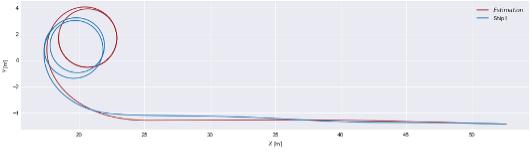
\includegraphics[width=0.8\textwidth]{./img/5-4.png}
    \caption{Sample data and split estimated results (180.00s – 245.50s)}
    \label{fig:5-4_png}
\end{figure}

\begin{figure}[htbp]
    \centering   
    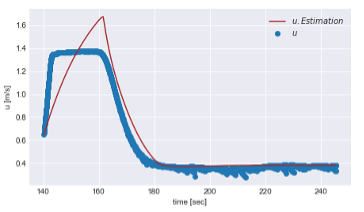
\includegraphics[width=0.8\textwidth]{./img/5-5.png}
    \caption{Sample data and split estimated results (180.00s – 245.50s)}
    \label{fig:5-5_png}
\end{figure}

\begin{figure}[htbp]
    \centering   
    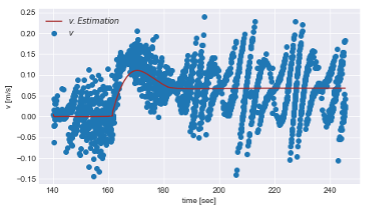
\includegraphics[width=0.8\textwidth]{./img/5-6.png}
    \caption{Sample data and split estimated results (180.00s – 245.50s)}
    \label{fig:5-6_png}
\end{figure}

\begin{figure}[htbp]
    \centering   
    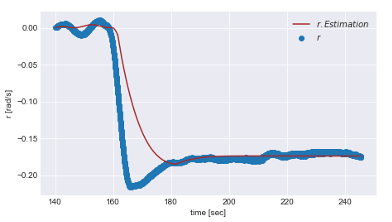
\includegraphics[width=0.8\textwidth]{./img/5-7.png}
    \caption{Sample data and split estimated results (180.00s – 245.50s)}
    \label{fig:5-7_png}
\end{figure}

\begin{table}[htbp]
 \caption{Evaluate results (case 1 \& case 5)}
 \label{tb:5-4}
 \centering
  \begin{tabular}{rrrrrrr}
    \toprule
    case & & 総走行距離 & 操舵前走行距離 & 最大縦距 & 最大横距 & 旋回半径 \\
    & & [m] & [m] & [m] & [m] & [m] \\
    \midrule
    \multirow{3}{*}{1} & 元データ & 67.13 & 26.68 & 8.57 & 4.72 & 2.21 \\
         & 推定データ        & 64.72 & 18.72 & 14.57 & 3.88 & 2.39 \\
         & 誤差[\%]        & 3.60 & 29.83 & 70.01 & 17.80 & 8.39 \\
    \midrule
    \multirow{3}{*}{2} & 元データ & 67.13 & 26.68 & 8.57 & 4.72 & 2.21 \\
         & 推定データ        & 67.78 & 27.70 & 7.39 & 5.40 & 2.39 \\
         & 誤差[\%]        & 0.96 & 3.83 & 13.77 & 14.41 & 8.39 \\
    \bottomrule
  \end{tabular}
\end{table}

それぞれの区間で操縦流体力微係数を推定した場合の推定航路は実際の35°旋回試験の航路に近い結果となった.特に操舵前の走行距離と最大縦距に大きな改善が見られた.総走行距離,旋回半径の誤差の結果より直進や旋回など針路が安定している区間の推定航路は精度よく表せられていると考えられるが,対して最大縦距・横距の誤差は15\%程度であり針路が安定している区間に比べ操舵直後の針路が安定していない区間の推定航路は精度よく表せられない結果となった.

\section{まとめ}
提案手法において操縦流体力微係数は旋回するときに生じる操縦性能の各種微係数であるという観点と運動方程式に最小二乗法を適用するという観点から最小二乗法適用区間は操縦運動パラメータが一定である区間を用いることとした.この提案した手法の妥当性は5.2.1.1でおこなった操舵直後の操縦運動パラメータが安定していない区間を用いて推定した結果が元データと大きく異なる挙動を示したFig. 5 2より確かめることができた. 

また,直進や舵角35°での旋回のような船体運動が異なる区間別でそれぞれ操縦流体力微係数を推定し,航路シミュレーションをおこなった結果は針路安定区間に比べ操舵直後の針路不安定区間の推定航路に多少の誤差がある結果となった.